\chapterwithauthor{Timothée Giet}{Krita Animation} 

\authorbio{Timothée Giet is a graphic artist from France, using exclusively free software since 2010. He works mainly on free software or freely licensed projects, doing all kinds of graphical work from illustration to icon design, and also teaching and creating training materials. He is a regular contributor to Krita and GCompris.}

\noindent{}Let me tell you the story about Krita and animation. For me, it started in 2010 when I discovered Krita. I was impressed by the quality of its drawing tools, and since I was looking for a free software alternative that would allow me to draw comics and animations, I secretly wished you could draw animations with it. 

Imagine how excited I was when, just the next year, a new mysterious contributor actually started working on an external plugin to add some animation tools. It was not easy to use nor very stable, but it was a good sign that other people wanted this. 

Around the same time, thanks to KDE e.V., I could attend the Libre Graphics Meeting where I met for the first time Boudewijn, the maintainer of Krita. During our conversation, I told him how great it would be if we could add some internal animation tools. It sounded a bit crazy at the time, and we both agreed that lot of work was needed first to get a solid drawing software, but the idea was there.

This first animation plugin experiments did not progress very much, and the main author left them unfinished. Later in 2013, a more serious project started with a Google Summer of Code student trying to add some internal animation tools. Sadly, even after two years, the plugin still was not production-ready and did not progress much. The contributions were still in a separate branch and not yet integrated in the main binary.

It was finally in 2015 that another Google Summer of Code student managed to really integrate the animation tools, learning from the mistakes in previous attempts. Now we have Krita 3.0, officially released and including basic animation tools. Animators from all over the world quickly started adopting it and sent some warm feedback.\todo{native speaker check - warm}

But this is only the beginning. We are still working on adding more tools and features, and I have no doubt that Krita will soon become a famous software tool in the animation world, if it hasn't already. It is a big step forward for people creating multimedia content exclusively with free software (for the operating system as for the tools). We now have a quite complete ecosystem of tools available in which Krita provides a missing piece for traditional animators. Let's see what people will create with it.

\begin{center}
 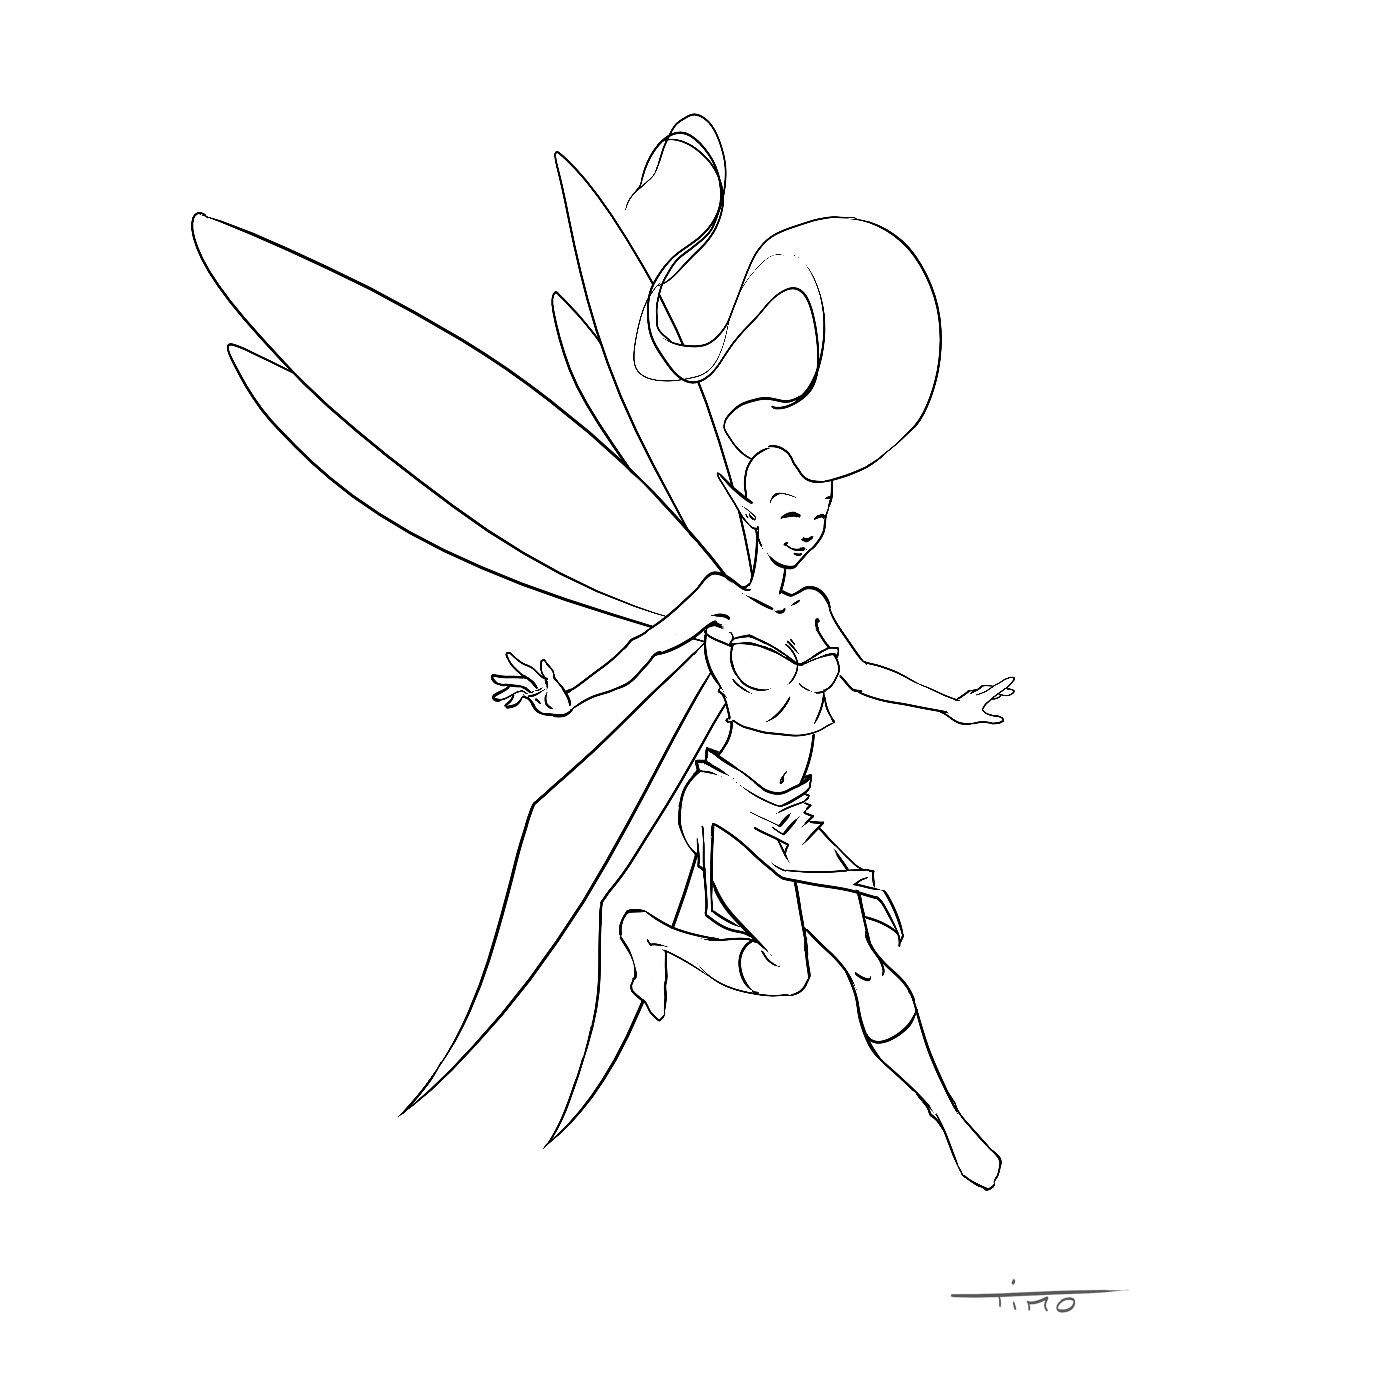
\includegraphics[scale=0.17,keepaspectratio=true]{./SeaFaery.png}
\end{center}
